        %%******************************************%%
        %%                                          %%
        %%        Modello di tesi di laurea         %%
        %%            di Andrea Giraldin            %%
        %%                                          %%
        %%             2 novembre 2012              %%
        %%                                          %%
        %%******************************************%%

\begin{document}
    \frontmatter
    \begin{titlepage}
    \begin{center}
        \begin{LARGE}
            \textbf{\myUni}\\
        \end{LARGE}

        \vspace{10pt}

        \begin{Large}
            \textsc{\myDepartment}\\
        \end{Large}

        \vspace{10pt}

        \begin{large}
            \textsc{\myFaculty}\\
        \end{large}

        \vspace{30pt}
        \begin{figure}[htbp]
            \centering
            
\includegraphics[height=6cm]{unipd-logo}
        \end{figure}
        \vspace{30pt}

        \begin{LARGE}
            \textbf{\myTitle}\\
        \end{LARGE}

        \vspace{10pt}

        \begin{large}
            \textsl{\myDegree}\\
        \end{large}

        \vspace{40pt}

        \begin{large}
            \begin{flushleft}
                \textit{Relatore}\\
                \vspace{5pt}
                \profTitle\ \myProf
            \end{flushleft}

            % You can tweak the spacing to have professor and student names on the same line
            % useful if the page is broken by a long thesis title and you need more space
            % \vspace{-52pt}

            \begin{flushright}
                \textit{Laureando}\\
                \vspace{5pt}
                \myName \\
                \vspace{5pt}
                \textit{Matricola} \myID
            \end{flushright}
        \end{large}

        \vspace{40pt}

        \line(1, 0){338} \\
        \begin{normalsize}
            \textsc{Anno Accademico \myAA}
        \end{normalsize}
    \end{center}
\end{titlepage}

    \clearpage
\phantomsection
\thispagestyle{empty}

\hfill
\vfill

\noindent\myName: \textit{\myTitle,}
\myDegree,
\textcopyright\ \myTime.

    \cleardoublepage
\phantomsection
\thispagestyle{empty}
\pdfbookmark{Dedica}{Dedica}

\vspace*{3cm}

\begin{center}
    If you really look closely, most overnight successes took a long time. \\ \medskip
    % Try not to become a man of success. Rather become a man of value. \\ \medskip --- Albert Einstein
    % Time waits for no one. \\ \medskip --- Unknown Author
    --- Steve Jobs
\end{center}

\medskip

\begin{center}
    Ai miei genitori
\end{center}

    \cleardoublepage
\phantomsection
\pdfbookmark{Sommario}{Sommario}
\begingroup
\let\clearpage\relax
\let\cleardoublepage\relax
\let\cleardoublepage\relax

\chapter*{Sommario}

Il presente documento descrive il lavoro svolto durante il periodo di stage, della durata di trecento ore, dal laureando Nicolò Pellegrinelli presso l'azienda Prorob S.r.l., con sede a Grisignano di Zocco (VI).\\
Il tirocinio si è sviluppato intorno allo studio dei metodi di autenticazione e autorizzazione alle risorse protette di un'applicazione web, con particolare attenzione all'uso di \emph{\gls{jwt}}\glsfirstoccur e dei protocolli adottati per garantire confidenzialità e integrità dei dati.\\
Questo studio è stato completato con l'implementazione di un \emph{ChatBot} per la piattaforma di messaggistica \emph{Microsoft Teams}, utilizzando gli strumenti studiati al fine di garantire sicurezza e autenticità dei dati scambiati.\\

%\vfill

%\selectlanguage{english}
%\pdfbookmark{Abstract}{Abstract}
%\chapter*{Abstract}

%\selectlanguage{italian}

\endgroup

\vfill

    \cleardoublepage
\phantomsection
\pdfbookmark{Ringraziamenti}{ringraziamenti}

% \begin{flushright}{
%     \slshape
%     ``Life is really simple, but we insist on making it complicated''} \\
%     \medskip
%     --- Confucius
% \end{flushright}


\bigskip

\begingroup
\let\clearpage\relax
\let\cleardoublepage\relax
\let\cleardoublepage\relax

\chapter*{Ringraziamenti}

\noindent \textit{Vorrei esprimere la mia profonda gratitudine al Prof. \myProf, relatore della mia tesi, per la sua disponibilità e il suo aiuto fornitomi durante la stesura del lavoro.}\\

\noindent \textit{Ringrazio con tanto affetto i miei genitori, che mi hanno sempre sostenuto e supportato in ogni mia decisione.}\\

\noindent \textit{Un ringraziamento speciale ai nonni, che con la loro curiosità hanno sempre motivato e sostenuto il mio percorso universitario}\\

\noindent \textit{Vorrei inoltre ringraziare tutti i miei amici, per questi fantastici anni ricchi di nuove avventure}\\
\bigskip

\noindent\textit{\myLocation, \myTime}
\hfill \myName

\endgroup

    \cleardoublepage
\pdfbookmark{\contentsname}{tableofcontents}
\setcounter{tocdepth}{2}
\tableofcontents
%\markboth{\contentsname}{\contentsname}
\clearpage

\begingroup
    \let\clearpage\relax
    \let\cleardoublepage\relax
    \let\cleardoublepage\relax

    % Figures list
    \phantomsection
    \pdfbookmark{\listfigurename}{lof}
    \listoffigures

    \vspace*{8ex}

    % Tables list
    \phantomsection
    \pdfbookmark{\listtablename}{lot}
    \listoftables

    \vspace*{8ex}
\endgroup

\cleardoublepage

    \cleardoublepage

    \mainmatter
    \chapter{Introduzione}
\label{cap:introduzione}


\section{L'azienda}

Lo stage è stato svolto presso la sede operativa di Prorob S.r.l. in Grisignano di Zocco (VI).


\section{Contesto}

Ogni giorno condividiamo una vasta quantità di informazioni personali e confidenziali attraverso vari servizi web, dai social network alle banche.
Queste informazioni, se non adeguatamente protette dai vari metodi di autenticazione, possono diventare bersagli facili di attacchi informatici.
Infatti ogni accesso a un account, ogni transazione online e ogni semplice login contengono dati che, se caduti nelle mani sbagliate, potrebbero causare danni significativi.

Da diversi anni, l'accesso a risorse online protette è diventato un processo molto frequente per la maggior parte delle persone e spesso non ci rendiamo conto di quanto sia importante proteggere le nostre credenziali di accesso.
Una password debole o riutilizzata può diventare l'elemento che un malintenzionato potrebbe sfruttare per accedere a informazioni sensibili.
E non è solo una questione di password: l'intero processo di autenticazione deve essere sicuro.

Questi metodi, oltre a verificare l'identità di un utente prima di consentire l'accesso alle risorse protette, devono anche garantire che i dati trasmessi durante il processo di autenticazione rimangano confidenziali e integri.
Ma quali sono i protocolli e le tecnologie che rendono tutto questo possibile? Come possiamo essere sicuri che le nostre informazioni siano davvero protette quando accediamo a un servizio online?

Lo stage si propone di realizzare uno studio in grado di rispondere a queste domande, analizzando l'autenticazione attraverso \emph{JSON Web Token (JWT)} e i protocolli necessari per garantire la completa sicurezza del processo di autenticazione.


\section{Organizzazione del documento}

\begin{description}
    \item[{\hyperref[cap:inquadramento-stage]{Il secondo capitolo}}] introduce lo stage, descrivendo il concetto di autenticazione e presentando l'idea del progetto.
    
    \item[{\hyperref[cap:autenticazione-jwt]{Il terzo capitolo}}] approfondisce l'utilizzo dell'autenticazione basata su \emph{\gls{token}}\glsfirstoccur di tipo \emph{JWT} e i protocolli necessari per garantire la loro sicurezza.
    
    \item[{\hyperref[cap:analisi-requisiti]{Il quarto capitolo}}] approfondisce ...
    
    \item[{\hyperref[cap:progettazione-codifica]{Il quinto capitolo}}] approfondisce ...
\end{description}

Riguardo la stesura del documento sono state adottate le seguenti convenzioni tipografiche:
\begin{itemize}
	\item gli acronimi, le abbreviazioni e i termini ambigui o di uso non comune menzionati vengono definiti nel glossario, situato alla fine del presente documento;
	\item per la prima occorrenza dei termini riportati nel glossario viene utilizzata la seguente nomenclatura: \emph{parola}\glsfirstoccur;
	\item i termini in lingua straniera o facenti parti del gergo tecnico sono evidenziati con il carattere \emph{corsivo}.
\end{itemize}

    \chapter{Inquadramento dello stage}
\label{cap:inquadramento-stage}

\intro{Lo stage, come anche questo documento, si divide in due parti. La prima parte si concentra sullo studio dei \emph{JWT}, metodi di firma e metodi di crittografia. La seconda parte riguarda invece l'implementazione di un \emph{ChatBot} per la piattaforma di messaggistica Microsoft Teams, utilizzando \emph{JWT} firmati e crittografati}\\

\section{Introduzione alla ricerca}
Il processo dell'autenticazione è l'atto di verificare le credenziali dell'utente in termini di correttezza o tempo\footcite{site:token-cookie-auth}.

Per correttezza si intende che le credenziali siano valide e che l'utente sia chi dice di essere.
Al momento dell'accesso, un token di autenticazione\footnote{In questo contesto, per token di autenticazione si intende una qualsiasi forma di credeziale di autentiazione.} viene assegnato all'utente.
Questo token viene utilizzato per verificare l'identità dell'utente in ogni richiesta successiva.

Per tempo, invece, si intende che l'utente abbia accesso al sistema per un periodo di tempo limitato.
Questo periodo di tempo è definito dal tempo di scadenza del token.
Quando il token scade, l'utente deve autenticarsi nuovamente per ottenere un nuovo token.

L'autenticazione è un processo fondamentale per la sicurezza di un'applicazione.
Essa, infatti, permette di verificare che l'utente sia chi sostiene di essere, dando ad ogni utente un'identità univoca che protegge i dati dell'utente stesso negando l'accesso a soggetti non autorizzati.

Esistono principalmente due metodi di autenticazione: l'autenticazione basata su \emph{\gls{web cookie}}\glsfirstoccur e l'autenticazione basata su token.

\subsection{Autenticazione basata su web cookie}
Un web cookie, o più semplicemente cookie, è un piccolo blocco di dati creato da un server web e inviato all'utente\footcite{site:cookie-wikipedia}.
Questi dati sono spesso essenziali per il funzionamento di un sito web, in quanto permettono di memorizzare, oltre alla sessione dell'utente, informazioni salvate dall'utente stesso, come le preferenze sull'aspetto grafico o gli articoli aggiunti al carrello.

L'utilizzo dei cookie per l'autenticazione è considerato l'approccio classico ed è spesso indicato come autenticazione basata su sessione. 
Questo perché il server li genera con un ID di sessione che memorizza nel proprio database e invia al client\footnote{Il client fa parte dell'architettura client-server ed è l'entità che richiede risorse o servizi da un server. Nel contesto delle applicazioni web, il client è tipicamente rappresentato dal browser web o da un'applicazione che l'utente utilizza per interagire con il server. Il client invia richieste al server e riceve risposte che possono includere dati, pagine web, file o altri contenuti.}.
Il client, ogni volta che fa una richiesta al server, invia il cookie con l'ID di sessione che il server utilizza per identificare l'utente, verificandone la validità.

L'autenticazione basata su cookie è considerata con stato (dall'inglese \emph{stateful}) in quanto sia il client che il server devono mantenere lo stato della sessione. \\

\noindent Il procedimento completo di autenticazione basata su cookie, illustrato in figura \ref{fig:auth-cookie-based}, è il seguente:
\begin{enumerate}
	\item L'utente che vuole accedere alla risorsa protetta inserisce le proprie credenziali.
	\item Il server verifica le credenziali e, se corrette, crea un cookie con un ID di sessione univoco.
	\item Il cookie viene inviato al client, il cui browser memorizza in modo automatico.
	\item Il client, ogni volta che fa una richiesta al server, invia il cookie con l'ID di sessione.
	\item Una volta verificato dal server, all'utente viene permesso l'accesso alla risorsa protetta.
	\item In caso di scadenza del cookie, l'utente deve autenticarsi nuovamente per ottenerne uno nuovo.
	\item Quando viene effettuato il logout, il cookie viene cancellato dal client e invalidato dal server.
\end{enumerate}

\begin{figure}[!ht] 
    \centering 
    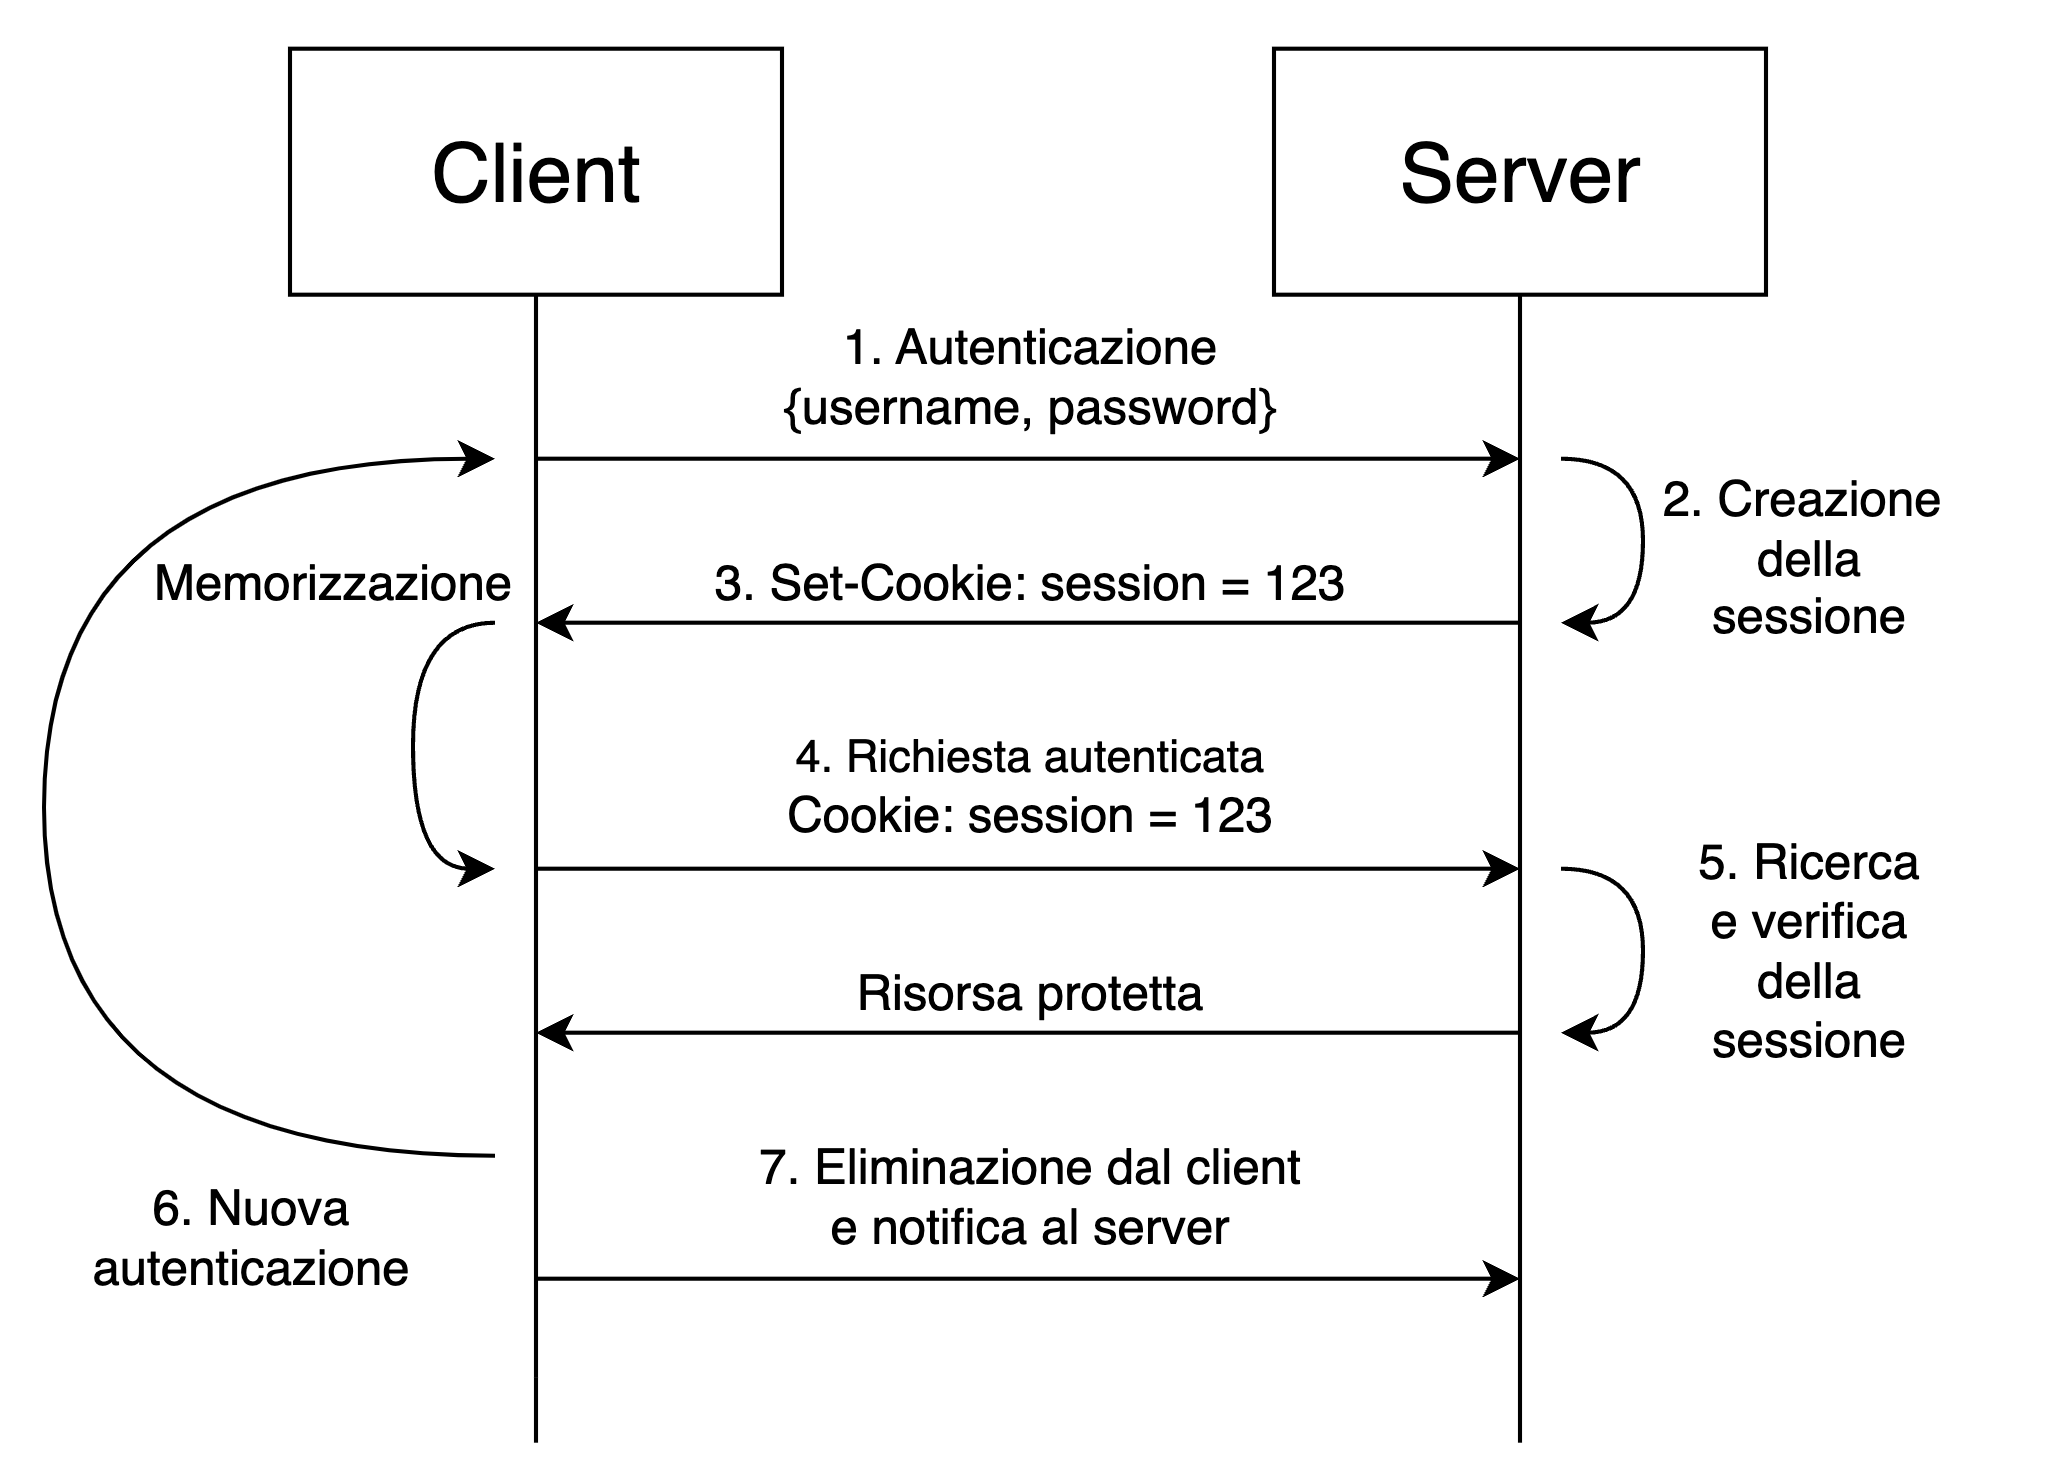
\includegraphics[width=0.9\columnwidth]{descrizione-stage/auth-cookie-based} 
    \caption{Processo di autenticazione basato su cookie}
	\label{fig:auth-cookie-based}
\end{figure}

\noindent L'utilizzo di cookie per l'autenticazione ha molti vantaggi.
Il principale è che sono supportati da tutti i browser e sono facili da implementare, in quanto è il browser stesso a gestirne la memorizzazione e l'invio.
I cookie inoltre necessitano di poca memoria e possono essere utilizzati anche per i \emph{sottodomini} di un sito web.

Tuttavia, l'autenticazione basata su cookie ha anche dei limiti.
Infatti, essi sono vulnerabili ad attacchi di tipo \emph{Cross-Site Scripting (XSS)} e \emph{Cross-Site Request Forgery (CSRF)} e non sono adatti per le architetture senza stato (dall'inglese \emph{stateless}), come alcuni tipi di \emph{\gls{API}}\glsfirstoccur.
Inoltre, i cookie non sono facilmente scalabili e non sono adatti per le applicazioni distribuite, in quanto dovrebbero essere memorizzati in un \emph{database} condiviso che potrebbe aumentare la complessità dell'applicazione.

\subsection{Autenticazione basata su token}
Un metodo di autenticazione alternativo all'utilizzo dei cookie è l'autenticazione basata su token.
Questo metodo è diventato molto popolare negli ultimi anni grazie all'aumento delle applicazioni web single page, al maggiore utilizzo di \emph{\gls{API RESTful}}\glsfirstoccur e dalla diffusione di dispositivi \emph{\gls{IoT}}\glsfirstoccur.

Un token è un oggetto simbolico rilasciato da un'autorità fidata\footcite{site:token-based-authentication-cloudflare}, ovvero il server, che permette all'utente di accedere a una risorsa protetta.
Diversamente dai cookie, i token sono \emph{stateless}, dunque non è necessaria la memorizzazione di alcuna informazione sul server.
Ciò è possibile perché ogni token contiene tutte le informazioni necessarie per la verifica dell'identità dell'utente e per l'accesso alla risorsa protetta. \\

\noindent Analogamente ai cookie, l'autenticazione basata su token viene effettuata nel seguente modo, come illustrato in figura \ref{fig:auth-token-based}:
\begin{enumerate}
	\item L'utente che vuole accedere alla risorsa protetta inserisce le proprie credenziali.
	\item Il server verifica le credenziali e, se corrette, genera un token con tutte le informazioni necessarie per l'accesso alla risorsa protetta.
	\item Il token viene inviato al client, il quale lo memorizza in modo sicuro.
	\item A questo punto, quando il client ha bisogno di accedere a una risorsa prottetta, include il token nella richiesta.
	\item Il server verifica la sua validità e consente l'accesso alla risorsa richiesta. 
	\item In caso di scadenza, l'utente deve autenticarsi nuovamente per ottenere un nuovo token.
	\item Quando viene effettuato il logout, il token viene cancellato dal client. Il server, invece, essendo senza stato, non ha bisogno di effettuare ulteriori operazioni.
\end{enumerate}

\begin{figure}[!ht] 
	\centering 
	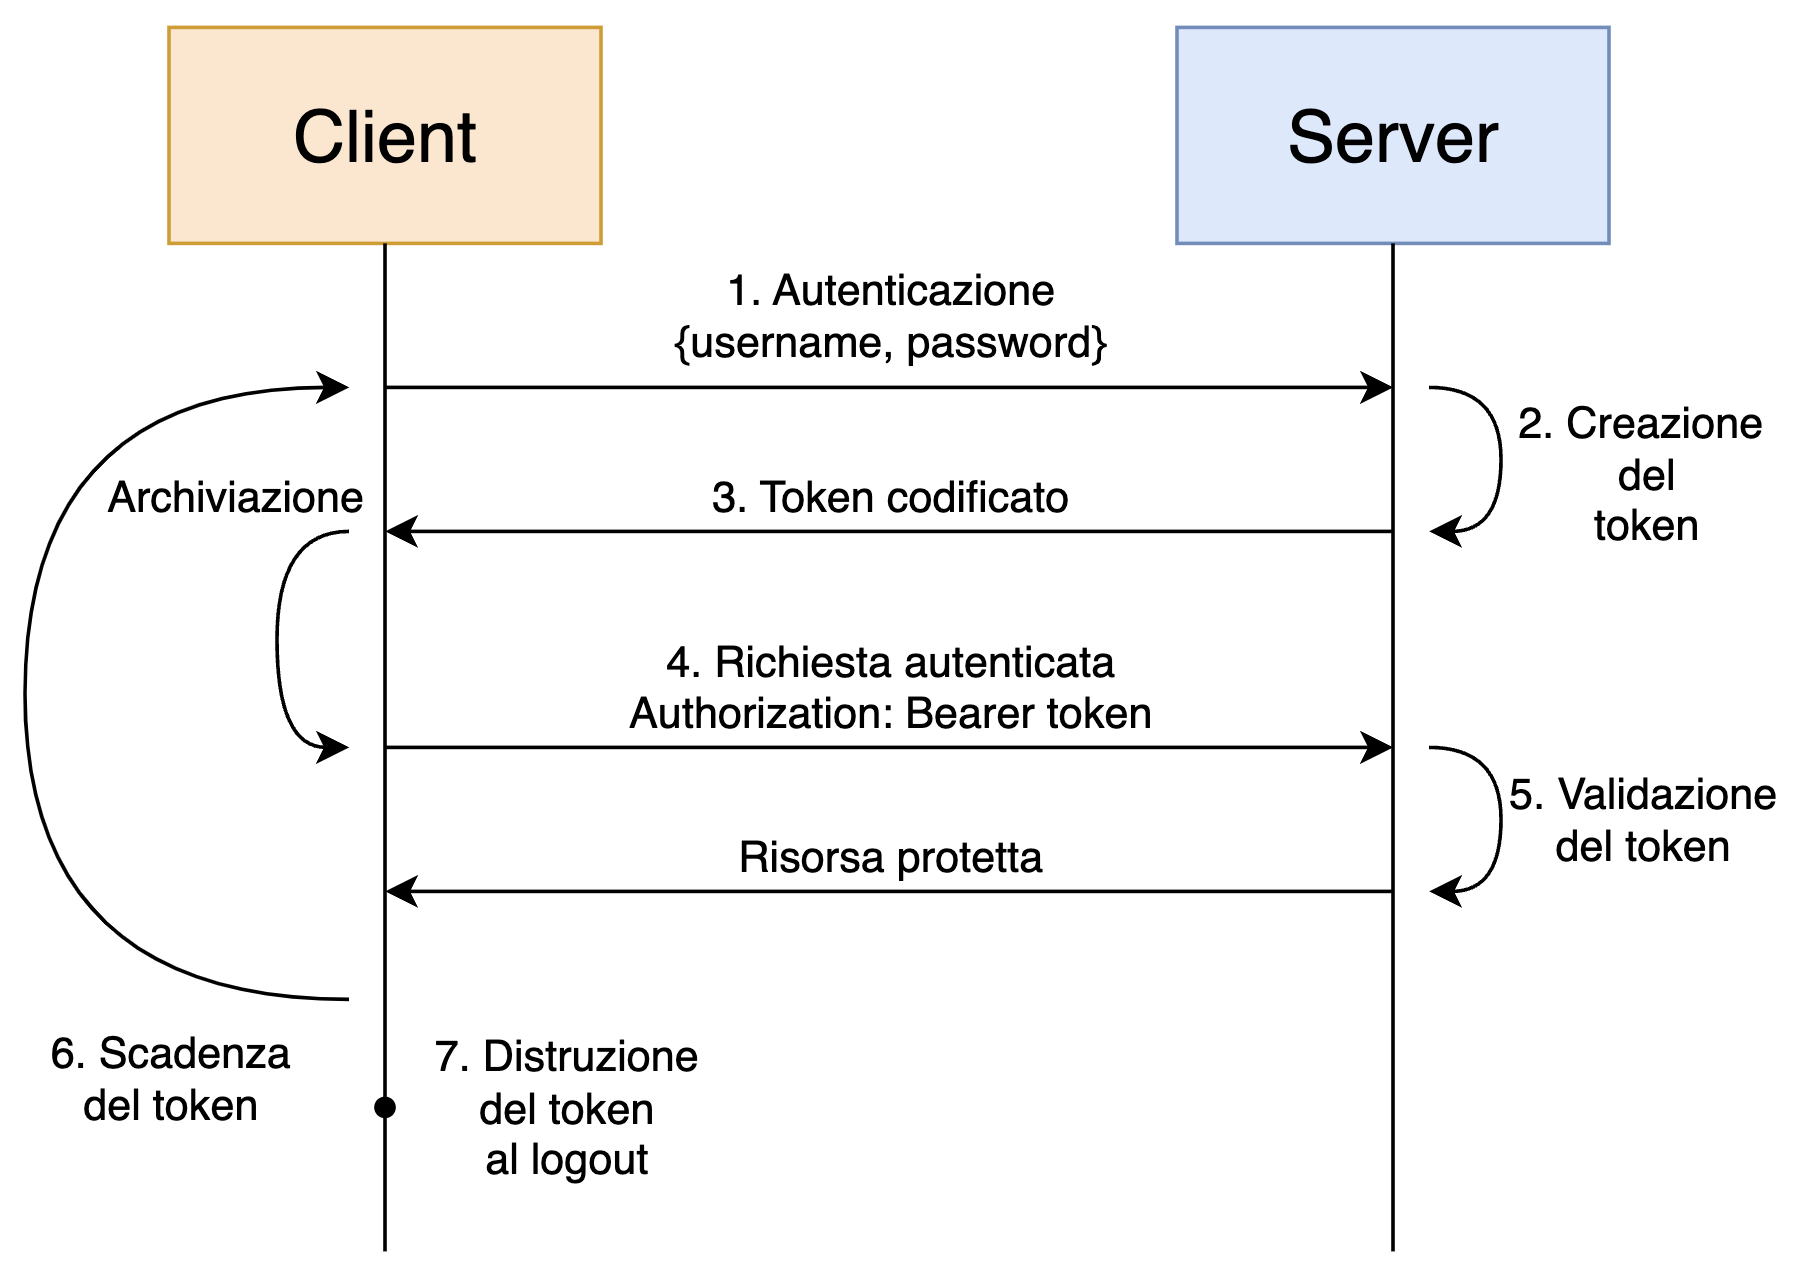
\includegraphics[width=0.9\columnwidth]{descrizione-stage/auth-token-based} 
	\caption{Processo di autenticazione basato su token}
	\label{fig:auth-token-based}
\end{figure}

\noindent L'utilizzo di questo metodo di autenticazione permette, dal lato server, di velocizzarne il processo, poiché non è necessaria nessuna verifica nel database.
Inoltre, la presenza di dati addizionali all'interno del token, come il livello dei permessi dell'utente, consente di semplificare ulteriormente il processo.
D'altro canto, questi campi addizionali aumentano notevolmente le dimensioni, rendendo la trasmissione e l'archiviazione più onerose.

Tuttavia, il più grande vantaggio dell'autenticazione basata su token è la possibilità di essere utilizzata anche per applicazioni mobili e \emph{API} che non si interfacciano con un browser.
I cookie, infatti, non si interfacciano correttamente con applicazioni native per dispositivi mobili, mentre i token possono essere facilmente integrati in qualsiasi applicazione con le stesse \emph{API}, se scritti correttamente.
In aggiunta, sono anche facilmente implementabili in applicazioni distribuite, come quelle per dispositivi \emph{IoT}.\\

\noindent Questo documento si concentra sull'autenticazione basata su token, in particolare su quelli di tipo \emph{JSON Web Token (JWT)}.


\section{Introduzione all'implementazione}
Uno dei vantaggi dell'utilizzo di metodi \emph{stateless} è la possibilità di integrarli facilmente in qualsiasi applicazione, indipendentemente dalla tecnologia utilizzata.
L'impossibilità di utilizzare i cookie senza l'ausilio di un browser rende i token la scelta migliore per applicazioni che utilizzano \emph{API RESTful}.

Per completare questo studio, è stato richiesto di implementare un \emph{ChatBot} in \emph{C\#} per la piattaforma di messaggistica Microsoft Teams utilizzando le \emph{API} di Microsoft Graph e token firmati e crittografati per garantire la sicurezza e la riservatezza di tutti i dati scambiati.

\subsection{Microsoft Teams}

\begin{figure}[!ht] 
	\centering 
	
\includegraphics[width=0.3\columnwidth]{descrizione-stage/logo-teams} 
	\caption{Logo di Microsoft Teams}
\end{figure}

Microsoft Teams\footcite{site:microsoft-teams} è una piattaforma di messaggistica e collaborazione offerta da Microsoft.
Essa consente a organizzazioni, team e singoli utenti di comunicare e collaborare con colleghi e clienti in tempo reale tramite chat, videoconferenze e chiamate.
Il \emph{ChatBot} implementato su questa piattaforma consentirà ai clienti di Prorob S.r.l di interagire con i servizi di Quindi Production Copilot in un modo più semplice e veloce.

\subsection{Microsoft Graph}

\begin{figure}[!ht] 
	\centering 
	
\includegraphics[width=0.3\columnwidth]{descrizione-stage/logo-graph} 
	\caption{Logo di Microsoft Graph}
\end{figure}

Microsoft Graph\footcite{site:microsoft-graph} è una piattaforma di sviluppo che unifica le \emph{API} di Microsoft 365 e Azure, permettendo alle applicazioni sviluppate da terze parti di interagire con i dati memorizzati nei vari servizi di Microsoft.
Utilizzando le \emph{API} di Microsoft Graph, il \emph{ChatBot} può interagire con con la chat di Teams, inviando messaggi e ricevendo notifiche.

\section{Obiettivi}
Prima dell'inizio dello stage Prorob S.r.l ha definito un piano di lavoro con gli obiettivi da raggiungere durante le 300-320 ore di stage. \\

\noindent Gli obiettivi principali prevedevano:
\begin{itemize}
	\item Studio dei \emph{JSON Web Token} e dei loro metodi di firma e di crittografia.
	\item Implementazione di una tecnologia generatrice di token \emph{API} firmati con certificati creati da chiavi ellittiche ed autenticati con metodologia \emph{HMAC}.
	\item Contribuire attivamente all'organizzazione e all'avanzamento delle attività in team.
\end{itemize}

Tuttavia, durante le settimane di stage, gli obiettivi iniziali sono stati rivisti in base alle esigenze emerse. Questo ha portato alla rimozione del un obiettivo e alla definizione di uno nuovo.
Infatti è stata rimossa l'implementazione della tecnologia generatrice di token \emph{API} firmati ed è stata sostituita con l'implementazione di un \emph{ChatBot} per la piattaforma di Microsoft Teams utilizzando i \emph{JWT} e algorithmi di firma e crittografia. \\

\noindent Gli obiettivi finali, dunque, sono stati:
\begin{itemize}
	\item Studio dei \emph{JSON Web Token} e dei loro metodi di firma e di crittografia.
	\item Implementazione di un \emph{ChatBot} per la piattaforma di messaggistica Microsoft Teams utilizzando i \emph{JWT} e algoritmi di firma e crittografia.
	\item Contribuire attivamente all'organizzazione e all'avanzamento delle attività in team.
\end{itemize}
    \chapter{Descrizione dello stage}
% \label{cap:descrizione-stage}

\intro{Breve introduzione al capitolo}\\

\section{Introduzione al progetto}

\section{Analisi preventiva dei rischi}

Durante la fase di analisi iniziale sono stati individuati alcuni possibili rischi a cui si potrà andare incontro.
Si è quindi proceduto a elaborare delle possibili soluzioni per far fronte a tali rischi.\\

\begin{risk}{Performance del simulatore hardware}
    \riskdescription{le performance del simulatore hardware e la comunicazione con questo potrebbero risultare lenti o non abbastanza buoni da causare il fallimento dei test}
    \risksolution{coinvolgimento del responsabile a capo del progetto relativo il simulatore hardware}
    \label{risk:hardware-simulator} 
\end{risk}

\section{Requisiti e obiettivi}


\section{Pianificazione}

    \chapter{Analisi dei requisiti}
\label{cap:analisi-requisiti}

\intro{Breve introduzione al capitolo}\\

\section{Casi d'uso}

Per lo studio dei casi di utilizzo del prodotto sono stati creati dei diagrammi.
I diagrammi dei casi d'uso (in inglese \emph{Use Case Diagram}) sono diagrammi di tipo \emph{UML} dedicati alla descrizione delle funzioni o servizi offerti da un sistema, così come sono percepiti e utilizzati dagli attori che interagiscono col sistema stesso.
Essendo il progetto finalizzato alla creazione di un tool per l'automazione di un processo, le interazioni da parte dell'utilizzatore devono essere ovviamente ridotte allo stretto necessario. Per questo motivo i diagrammi d'uso risultano semplici e in numero ridotto.

\begin{figure}[!h] 
    \centering 
    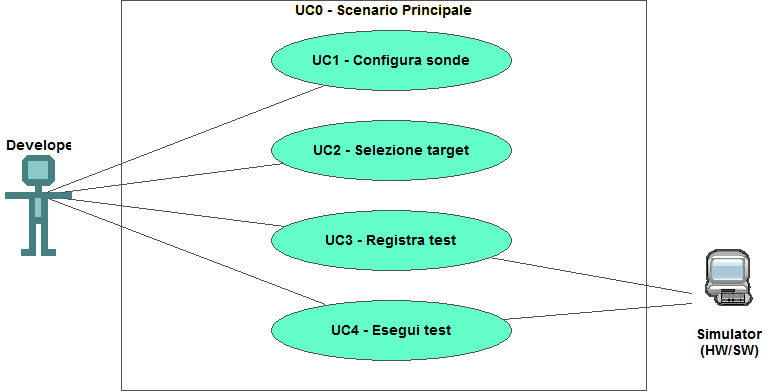
\includegraphics[width=0.9\columnwidth]{usecase/scenario-principale} 
    \caption{Use Case - UC0: Scenario principale}
\end{figure}

\begin{usecase}{0}{Scenario principale}
\usecaseactors{Sviluppatore applicativi}
\usecasepre{Lo sviluppatore è entrato nel plug-in di simulazione all'interno dell'IDE}
\usecasedesc{La finestra di simulazione mette a disposizione i comandi per configurare, registrare o eseguire un test}
\usecasepost{Il sistema è pronto per permettere una nuova interazione}
\label{uc:scenario-principale}
\end{usecase}

\section{Tracciamento dei requisiti}

Da un'attenta analisi dei requisiti e degli use case effettuata sul progetto è stata stilata la tabella che traccia i requisiti in rapporto agli use case.\\
Sono stati individuati diversi tipi di requisiti e si è quindi fatto utilizzo di un codice identificativo per distinguerli.\\
Il codice dei requisiti è così strutturato R(F/Q/V)(N/D/O) dove:
\begin{enumerate}
	\item[R =] requisito
    \item[F =] funzionale
    \item[Q =] qualitativo
    \item[V =] di vincolo
    \item[N =] obbligatorio (necessario)
    \item[D =] desiderabile
    \item[Z =] opzionale
\end{enumerate}
Nelle tabelle \ref{tab:requisiti-funzionali}, \ref{tab:requisiti-qualitativi} e \ref{tab:requisiti-vincolo} sono riassunti i requisiti e il loro tracciamento con gli use case delineati in fase di analisi.

\newpage

\begin{table}%
\caption{Tabella del tracciamento dei requisti funzionali}
\label{tab:requisiti-funzionali}
\begin{tabularx}{\textwidth}{lXl}
\hline\hline
\textbf{Requisito} & \textbf{Descrizione} & \textbf{Use Case}\\
\hline
RFN-1     & L'interfaccia permette di configurare il tipo di sonde del test & UC1 \\
\hline
\end{tabularx}
\end{table}%

\begin{table}%
\caption{Tabella del tracciamento dei requisiti qualitativi}
\label{tab:requisiti-qualitativi}
\begin{tabularx}{\textwidth}{lXl}
\hline\hline
\textbf{Requisito} & \textbf{Descrizione} & \textbf{Use Case}\\
\hline
RQD-1    & Le prestazioni del simulatore hardware deve garantire la giusta esecuzione dei test e non la generazione di falsi negativi & - \\
\hline
\end{tabularx}
\end{table}%

\begin{table}%
\caption{Tabella del tracciamento dei requisiti di vincolo}
\label{tab:requisiti-vincolo}
\begin{tabularx}{\textwidth}{lXl}
\hline\hline
\textbf{Requisito} & \textbf{Descrizione} & \textbf{Use Case}\\
\hline
RVO-1    & La libreria per l'esecuzione dei test automatici deve essere riutilizzabile & - \\
\hline
\end{tabularx}
\end{table}%

    \chapter{Progettazione e codifica}
\label{cap:progettazione-codifica}

\intro{Breve introduzione al capitolo}\\

\section{Tecnologie e strumenti}
\label{sec:tecnologie-strumenti}

Di seguito viene data una panoramica delle tecnologie e strumenti utilizzati.

\subsection*{Tecnologia 1}
Descrizione Tecnologia 1.

\subsection*{Tecnologia 2}
Descrizione Tecnologia 2

\section{Ciclo di vita del software}
\label{sec:ciclo-vita-software}

\section{Progettazione}
\label{sec:progettazione}

\subsubsection{Namespace 1} %**************************
Descrizione namespace 1.

\begin{namespacedesc}
    \classdesc{Classe 1}{Descrizione classe 1}
    \classdesc{Classe 2}{Descrizione classe 2}
\end{namespacedesc}


\section{Design Pattern utilizzati}

\section{Codifica}

    \chapter{Verifica e validazione}
\label{cap:verifica-validazione}

    \chapter{Considerazioni finali}
\label{cap:conclusioni}

\section{Risultati ottenuti}

Nonostante gli obiettivi iniziali non siano stati definiti in modo chiaro e siano stati quindi modificati durante il corso dello stage, il lavoro svolto è stato completato con successo e ha prodotto buoni risultati.
Infatti, l'implementazione originale della tecnologia generatrice di token \emph{API} firmati con certificati creati da chiavi ellittiche ed autenticati con metodologia \emph{HMAC} non è stata portata a termine.
Tuttavia, è stata sostituita con l'implementazione del \emph{ChatBot} per Microsoft Teams.

\noindent Tra i prodotti finali del tirocinio possiamo trovare:
\begin{itemize}
	\item Un documento che riassume il funzionamento dei token \emph{JWT} e degli algoritmi utilizzati per la creazione della firma digitale e della loro trasmissione sicura.
	\item Un \emph{ChatBot} per Microsoft Teams in grado di gestire diverse richieste contemporaneamente in totale sicurezza.
	\item Diversi piccoli script in \emph{Python} realizzati per contribuire alle esigenze dell'azienda e per facilitare il lavoro dei colleghi.
\end{itemize}

\section{Competenze acquisite}

Durante il tirocinio ho avuto l'opportunità di approfondire le mie conoscenze e di acquisirne di nuove.

Questa esperienza mi ha permesso di comprendere meglio il funzionamento di un'azienda e di come viene organizzato il lavoro al suo interno, sia individualmente che in gruppo.

Inoltre, ho approfondito le mie conoscenze in ambito di sicurezza informatica.
Ho scoperto che i processi di autenticazione, generalmente trasparenti per l'utente, sono molto più complessi di quanto si possa immaginare, ma sono fondamentali per garantire la privacy.

Infine, lavorare con nuove tecnologie, come \emph{Microsoft Teams} e \emph{Microsoft Graph}, e nuovi linguaggi di programmazione, come \emph{C\#}, ha ampliato il mio bagaglio di competenze informatiche.

\section{Valutazione personale}

Credo fermamente che l'esperienza di stage sia stata molto positiva e formativa.
Mi ha permesso di crescere sia professionalmente che personalmente, grazie all'ambiente aziendale dinamico e alla collaborazione con colleghi esperti e disponibili.

Sono convinto che le conoscenze acquisite nell'ambito della sicurezza informatica mi saranno molto utili in futuro, in quanto è un campo in continua evoluzione in cui è necessario avere una formazione di base solida.
Grazie alla creazione del \emph{ChatBot} ho potuto mettere in pratica queste conoscenze e apprendere un nuovo linguaggio di programmazione.

Infine, ritengo che il lavoro svolto abbia portato a buoni risultati e che il \emph{ChatBot} realizzato possa essere un valido strumento per l'azienda.

Il buon rapporto con i colleghi e la soddisfazione dell'azienda per la collaborazione degli scorsi mesi mi spingono a pensare che il mio contributo sia stato apprezzato e che il lavoro svolto sia stato di qualità.

    % \appendix
    % \chapter{Appendice A}

\epigraph{Citazione}{Autore della citazione}


    \backmatter
    % \printglossary[type=\acronymtype, title=Acronimi e abbreviazioni, toctitle=Acronimi e abbreviazioni]
    \printglossary[type=main, title=Glossario, toctitle=Glossario]

    \cleardoublepage
\chapter{Bibliografia}

\nocite{*}

% Print book bibliography
\printbibliography[heading=subbibliography,title={Riferimenti bibliografici},type=book]

% Print site bibliography
\printbibliography[heading=subbibliography,title={Siti web consultati},type=online]

\end{document}
